The simulation framework provides all needed functionalities to orchestrate a peer-to-peer network where the nodes are running the Bitcoin reference implementation.
The whole simulation runs on a single host using the virtualisation software \textit{Docker}.
The framework furthermore coordinates the block discovery in the network.
Based on a sequence defined in a configuration file the software sends commands to the nodes which are then generating valid blocks.
To be able to create blocks the nodes are executed in the \textit{regtest mode}, where the CPU-heavy proof-of-work is disabled, and the nodes are accepting a RPC-call from outside which lets them create a new block immediately.
After a simulation run, the software parses the logs produced by the nodes and based on them the software generates a report which displays the key metrics of the simulation.

\todo[inline]{this should remain an introduction to the whole chapter (as all other chapters have an introductional paragraph). i extended the tick chapter and added the virtualisation chapter to explain why we did what.}

%The remaining of this chapter starts with the sub-chapter \ref{chap:tick}, where the general concept of a tick is introduced.
%Afterwards in the chapter \ref{chap:config_files} the different configuration files are explained.
%In the chapter \ref{chap:simulation} the whole procedure of a simulation with the three main steps preparation, execution and post-processing is explained.
%Lastly, in the chapter \ref{chap:commands} the implemented commands to execute the simulation framework are listed.
  
\section{Tick}
\label{chap:tick}

A fundamental concept of the simulation framework is a so-called tick.
A tick represents a small time span containing information about which nodes should find a new block in this tick.
Hence a tick forms an abstraction of a certain time span in the real time.
All blocks which should be generated in this time span are aggregated into the corresponding tick.
Since all blocks created in the same tick are considered to be created at the same time, a tick should never contain the information that one node creates multiple blocks.
This fact is also respected by the script creating the \textit{ticks.csv} explained in chapter \ref{chap:ticks_command}.

For a simulation run, multiple ticks are combined forming a sequence of ticks.
In combination with two other configuration files, the tick sequence builds the simulation scenario for a particular simulation run.
The exact duration of a tick is defined on execution time of the simulation and determines the actual speed of the simulation.

The concept of a tick helps to have an upper bound for the simulation speed.
This upper bound of a certain simulation scenario is reached when the execution time of at least one tick last longer than the tick duration itself.
In that case, the temporal succession of the block events is disturbed, which can result in inaccurate or wrong results.
In such a case the simulation speed should be lowered or the simulation scenario should be changed.

Additionally, the usage of ticks would allow to speed up the simulation by cutting out empty ticks or ticks which do not influence the investigated results of the simulation.
In that case, it needs to be defined when a certain event in a tick is over.
For example, block events can be considered to be over when all nodes received the whole block or heard about the block but did not requested it.
If such a block event is over, all subsequent ticks until the next tick with a block event could be ignored because those ticks would not influence block related simulation results.
Currently, such a mechanism is not implemented and therefore no ticks of a simulation scenario are ignored even though they are empty and would not influence the results.

\todo[inline]{actually skipping ticks or to know when a tick is over is the huge advantage of the tick concept right? i know network simulators only superficial but they use the same concept and can speed up the simulation because they know when a the events are over, right? in our case we would need to know when the block finished to propagate then we could immediately go to the next tick. i think we discussed this already once! but yes, i hope i explained the concept of ticks and how we use them well!}

\section{Virtualisation}
\label{chap:virtualisation}

The simulation framework virtualises the whole peer-to-peer network on one single host by using \textit{Docker}.
The software \textit{Docker} runs the nodes as so-called containers, which are using the functionalities of the same kernel in an isolated manner.
Hence, they do not interfere each other as long as the host system provides enough resources to them.
In the case that the host system is under-provisioned and does not provide enough resources to the nodes, the simulation results may be distorted.
To resolve that problem the simulation scenario needs to be simplified or a better host machine needs to be used.

The virtualisation of the network on one host machine has the advantage of an easy and manageable setup.
As long as the host machine can scale vertically with the defined simulation scenario, there is no need to deploy a physically peer-to-peer network to simulate the scenario.
Furthermore, since all nodes rely on the same kernel functionalities also all nodes use the same system time.
This is especially helpful for the aggregation of the log files of all different containers because it assures that the timestamps in the log lines actually happened in exactly this order.

Other simulation technologies are not using virtualisation features and simulate the peer-to-peer networks with more abstract models such as numeric simulations and MDP's \cite{eyal2014majority, bahack2013theoretical, gervais2015tampering, nayak2016stubborn, sapirshtein2016optimal, gervais2016security}. Compared to these simulation technologies the introduced simulation framework has the advantage that already existing implementations, as in the case of this thesis the Bitcoin reference implementation, can be reused directly.
Hence, there is no significant implementation effort needed to simulate a certain blockchain protocol and the simulations reflect all implementation details by relying directly on the implemented code.

\section{Configuration files}
\label{chap:config_files}

A simulation executed by the software needs to be configured with the configuration files \textit{nodes.csv}, \textit{network.csv} and \textit{ticks.csv}.
The configuration files are stored in the concise CSV format and on a specific location on the disk to be processed by the simulation framework.
The usage of configuration files as input for a simulation provide the flexibility that they can be written manually, that they can be generated by a small script or a combination of both.
For example, a small script generates a needed configuration file.
Afterwards, the user can adjust the configuration file by editing it and does not need to implement an own script for the specific scenario but does also no need to write the whole configuration file by hand.
Furthermore, the created configuration files can be copied to the output directory of a simulation run providing an easy method to preserve all input parameters used for the run.

The simulation framework already implements for each configuration file a simple script which can be executed by the corresponding commands \textit{nodes} (chapter \ref{chap:nodes_command}), \textit{network} (chapter \ref{chap:network_command}) and \textit{ticks} (chapter \ref{chap:ticks_command}).

\subsection{\textit{nodes.csv}}

The \textit{nodes.csv} contains the configuration of every node which should be orchestrated by the simulation framework.
Each row in the file reflects one node consisting of:
\begin{itemize}
	\item \textit{node\_type}: Either \textit{bitcoin} if the node is a normal node or \textit{selfish} if the node should act like a selfish node.
	\item \textit{share}: The computation power proportion of the node in the network.
	\item \textit{docker\_image}: The \textit{Docker} image to use for the node.
	\item \textit{latency}: The latency  of the node in the peer-to-peer network.
	The node will have this latency to all other nodes with the exact same latency.
	For other connections, the two different latencies are added.
	Hence, two nodes, one node with 100 milliseconds of latency and one node with 50 milliseconds, will have 150 milliseconds of latency between each other during the simulation.
	\item \textit{group}: Which group the node did belong to during the creation of the \textit{nodes.csv} by the script introduce in chapter \ref{chap:commands}.
	The parameter group is ignored during the actual execution of the simulation.
\end{itemize}
 
\subsection{\textit{network.csv}}
The \textit{network.csv} reflects a connection matrix as shown in table \ref{tab:network_csv}.
The simulation framework starts each node in a way that a node on the y-axis tries to establish an outgoing connection to another node on the x-axis whenever the corresponding value in the matrix is 1.

\begin{table}
  \centering
  \begin{tabular}{c|ccc}
    			& node a 	& node b	& node c	\\
    \hline
    node a		& 0			& 1         & 0         \\
    node b      & 0         & 0         & 1			\\
    node c      & 1         & 1			& 0         \\
  \end{tabular}
  \caption{An example \textit{network.csv} represented as table}
  \label{tab:network_csv}
\end{table}

\subsection{\textit{ticks.csv}}

The \textit{ticks.csv} contains all ticks which should be executed by the simulation framework.
Each line represents a tick with no, one or multiple block events.
Hence the length of lines in a \textit{ticks.csv} varies depending on the number of block events in the corresponding tick.

\section{Simulation}
\label{chap:simulation}

The main functionality of the simulation framework is to coordinate a simulation based on the configuration files.
The software uses therefore the high-level programming language \textit{Python} and the virtualisation software technology \textit{Docker}.
\textit{Python} is mainly used to handle the configuration files and to execute \textit{Docker} and other binaries whenever necessary automatically.
\textit{Docker} on the other side provides the needed capabilities to run the Bitcoin reference implementation and other programs in lightweight containers on one single host as explained in chapter \ref{chap:virtualisation}.
	
To execute a simulation the command \textit{simulate} (chapter \ref{chap:simulate_command}) can be used.
In that case, the configuration files need to be available on disk.
The commands \textit{run} (chapter \ref{chap:run_command}) and \textit{multi-run} (chapter \ref{chap:multi_run_command}) provide another possibility to execute a simulation, creating all configuration files before starting the simulation.
The simulation itself can be split up into the three phases preparation, execution and post-processing.

\begin{figure}[t]
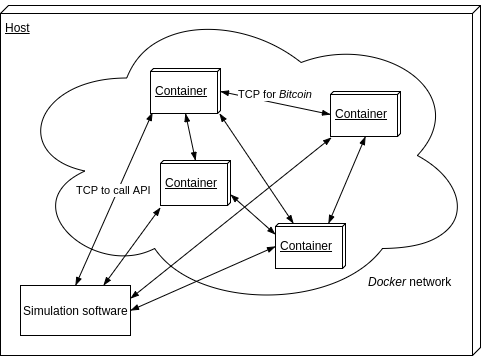
\includegraphics[width=8cm]{overview_setup}
\centering
\caption{Overview of the virtual peer-to-peer network}
\label{fig:overview}
\end{figure}

\subsection{Preparation}

The preparation phase is the first phase of a simulation run.
At the beginning, a simulation directory is created and all configuration files are copied into the new directory to assure reproducibility.
Subsequently, a virtual peer-to-peer network is assembled as depicted in figure \ref{fig:overview}.
Therefore firstly a \textit{Docker} network with the driver set to \textit{bridge} is created which under the hood configures a new network interface in the networking stack of the host machine.
This network interface is used by the \textit{Docker} containers to connect and communicate to other containers.
Afterwards based on the two configuration files \textit{nodes.csv} and \textit{networking.csv} the nodes are created as \textit{Docker} containers with \textit{bitcoind} set as command to be executed in the container.
Listing \ref{lst:docker_create} shows how \textit{Docker} is used to create a container, which executes \textit{bitcoind} on start-up.
In line 2 the unique IP of the container is set by using the \textit{-{}-ip} argument.
Line 3 shows the usage of a so-called \textit{Docker volume} to mount the folder \textit{data/run-10/node-5/} into the container's folder \textit{/data/regtest}.
By running \textit{bitcoind} in \textit{regtest mode} (line 6) and setting the data directory of \textit{bitcoind} to \textit{/data} (line 7) Bitcoin persists all relevant data into \textit{/data/regtest}.
Hence all the data persisted by \textit{bitcoind} under \textit{/data/regtest} will actually be persisted under \textit{data/run-10/node-5/} on the host machine and is therefore still available after the destruction of the container.
In line 8 we define to which other nodes the node should connect to by specifying their IP.
By using the \textit{-connect} parameters the Bitcoin reference implementation automatically stops to listen for incoming connections.
Since this is needed to accept incoming connections, it is re-enabled in line 9 by setting \textit{-listen} to 1.

Lastly, after all nodes are spawned, an RPC-connection to the Bitcoin API running in each node is established by using the library \textit{python-bitcoinlib}.
These connections are later used to directly send commands to the nodes.

\begin{minipage}{\linewidth}
\begin{lstlisting}[caption=Simplified version of how a node is started with \textit{Docker} and \textit{bitcoind}, label={lst:docker_create}, basicstyle=\ttfamily, captionpos=b]
docker run
	--ip=240.1.0.5
	--volume data/run-10/node-5:/data/regtest
	bitcoind_image
		bitcoind
			-regtest
			-datadir=/data
			-connect=240.1.0.2 -connect=240.1.0.9
			-listen=1
\end{lstlisting}
\end{minipage}
	
\subsection{Execution}
\label{chap:simulation_execution}

In the execution phase, the simulation framework iterates over each tick from the \textit{ticks.csv}.
If a tick contains a block event, the framework calls \textit{generate} on the Bitcoin API of the specific node to generate a new block.
Since all nodes are running in \textit{regtest mode} the proof-of-work is deactivated and the block can be created immediately.
Some ticks may contain multiple block events.
In this case, the block events are executed one after another always waiting for the block hash to be returned by the nodes.
The sequential execution of the block events is preferred over a parallelisation, which would introduce a new source of uncontrollable indeterminism making the results harder to reproduce even on the same host.

A simulation run is always executed with a certain tick duration.
This tick duration specifies how long a tick should last in real time.
Therefore the simulation framework simply keeps track of the passed time during the execution of the block events and sleeps afterwards until the tick is over.
If the completion of the block events lasts longer then the tick duration, then the framework immediately starts with the next tick and tries to regain the lost time.
The case where the execution of block events last longer than the tick duration, should be a rare exception.
If this happens more frequent the simulation scenario is configured too fast, which likely creates inaccurate results as explained in chapter \ref{chap:tick}.
Thus, the defined scenario should be created with fewer block events per tick or a higher tick duration should be configured for the simulation run.
The simulation framework itself states the number of exceptions of this type in the final report.

During the execution of the ticks, a thread separately collects information about the current CPU and memory usage.
For the CPU usage, the thread queries periodically the \textit{/proc/stat} file which is showing how much time the CPU spent in a certain state. 
The collected snapshots can later be used to determine the actual utilization of the CPU by calculating the differences between the snapshots.
For the memory usage, the thread reads periodically the \textit{MemAvailable} in \textit{/proc/meminfo} file.
This value provides a heuristic of the currently available memory on the machine.

\subsection{Post-processing}

The post-processing phase is the last phase of a simulation run.
At the beginning of this phase the consensus chain, denoting the longest chain of blocks all nodes agree about, is calculated.
This is done by starting at block height one and asking each node for the hash of the block on this height in their longest chain.
If all nodes have a block at this height and the hashes of all blocks are the same, then all nodes reached consensus and the block is added to the consensus chain.
In the next step, the height is increased by one and the previously described check is repeated.
If one node has no block at a certain height or the hashes of the blocks differ then the calculation of the consensus chain stops.

After the calculation of the consensus chain, all \textit{Docker} nodes are stopped and removed.
Because a separate data directory was mounted on each node by using \textit{Docker volumes} all relevant data, especially the log files, are still available on the host machine after the deletion of the \textit{Docker} nodes.
In the next step lines of the logs from nodes and from the log file of the simulation framework are parsed to retrieve information about the simulation run.
These log line types are:

\begin{itemize}
   \item \textit{BlockGenerateLine}: Log line produced by a node when a new block is generated.
   \item \textit{BlockStatsLine}: A log line displaying various information like block size about a freshly generated block.
   \item \textit{UpdateTipLine}: Log line produced by a node whenever a block updates a tip of the chain.
   \item \textit{PeerLogicValidationLine}: Log line produced when the proof-of-work of a received compact block is checked.  
   \item \textit{BlockReconstructLine}: A log line created when a compact block was successfully reconstructed.
   \item \textit{BlockReceivedLine}: Log line created when a node receives a normal block.
   \item \textit{TickLine}: A log line with information about an executed tick.
   \item \textit{BlockExceptionLine}: Log line created whenever the simulation framework was not able to successfully execute a block event.
   \item \textit{RPCExceptionEventLine}: Log line denoting an exception occurred while using the RPC-connection to a node.
\end{itemize}

The log lines \textit{BlockGenerateLine}, \textit{BlockStatsLine}, \textit{UpdateTipLine}, \textit{PeerLogicValidationLine}, \textit{BlockReconstructLine} and \textit{BlockReceivedLine} are all produced by nodes executing Bitcoin where on the other hand \textit{TickLine}, \textit{BlockExceptionLine} and \textit{RPCExceptionEventLine} are created by the simulation framework itself.
Furthermore, the \textit{BlockGenerateLine} log line was added especially for the simulation framework to the Bitcoin reference implementation.
Normally the reference implementation does not create a log line containing the block hash when it creates a new block.
To circumvent this fact, a log line was added to the reference implementation to persist the event of the block creation including a hash of the block.

The simulation framework persists all parsed log lines into CSV files where each log line type gets its file.
Subsequently, the \textit{preprocess.R} script prepares the CSV files for the final report creation.
When a simulation is executed a parameter can be passed which denotes how many ticks at the beginning and at the end should not be evaluated in the post-processing phase (\textit{skip\_ticks}).
The \textit{R} script then figures out when the first and the last tick to be evaluated occurred and tailors the log line types \textit{BlockGenerateLine} and \textit{BlockStatsLine} respectively.
All other types do not need to be tailored because they either are used to calculate some combined statistics like the block propagation time or because the statistics of these types are still calculated over the whole simulation duration like the memory usage.
The \textit{skip\_ticks} parameter allows the user to discard ticks which may created distorted data.
Right after the start it is likely that the nodes behave differently because the execute some initializing routines or run faster because they just started up.
At the end of the simulation run, it makes sense to ignore some ticks because blocks created at the end of the simulation would distort the analysis of the simulation.
Those blocks probably propagate faster, because right after them no other competing blocks are created.
Another problem could be that the simulation frameworks already starts to shut down the peer-to-peer network even though some blocks are still transmitted to other nodes.
How many ticks should be omitted depends on the simulation scenario and the right amount is difficult to determine.
An additional mitigation is to extend the overall simulation, which would reduce the influence of the distorted data from the first and last ticks.

Additionally, by omitting some ticks, the \textit{preprocess.R} script sorts all CSV files according to the timestamp of the log line.
This is necessary because the parsing of the log files is implemented in a multi-threading manner and thus the ordering from the original log files is lost.

After all CSV files are created the simulation frameworks generates a report by executing an \textit{R Markdown} file.
The final report contains:
\begin{itemize}
	\item general information about the simulation like the start and end time
	\item specifications and settings of the host machine used in the simulation
	\item all input arguments passed to the simulation
	\item summary of planned, executed and parsed block events
	\item overview of the duration of each phase of the simulation
	\item chart visualizing CPU and memory utilization
	\item chart showing the duration of a tick over time
	\item charts and information about blocks created during the simulation
	\item charts and information about exceptions happened during the simulation
\end{itemize}

Most of the stated information and charts can be directly generated from the CSV files with respective R commands.
Only the stale block rate and the propagation time of blocks need some further processing, which is executed on report creation.
\todo[inline]{stale block rate is explained in state-of-the-art. you mentioned to cite Bitcoin NG by Eyal. i did not found anything about stale block rate in that paper}

The stale rate, describing how many blocks did not end up in the longest chain, is calculated by checking each created block against the consensus chain determined previously by simply merging the \textit{BlockGenerateLine} log lines with the consensus chain.
The propagation time of blocks is calculated with \textit{R} as shown in listing \ref{lst:propagation_time}.
First, the \textit{BlockGenerateLine} log lines are merged with the lines describing the event of receiving a block, namely	\textit{UpdateTipLine}, \textit{PeerLogicValidationLine}, \textit{BlockReconstructLine} and \textit{BlockReceivedLine} creating a new data frame.
Since for example, \textit{UpdateTipLine} is also logged by the node which created the block in line 5 all these elements are filtered out of the data frame.
Afterwards, the data set is grouped by the block hash and the name of the node (line 7).
By filtering out the element with the lowest timestamp, the data frame now represents the points in time when a node heard first about a certain block.
Lastly, the propagation time is calculated by subtracting the timestamp of the \textit{BlockGenerateLine} log line from the timestamp of the receiving log lines.

\begin{minipage}{\linewidth}
\begin{lstlisting}[caption=Calculation of propagation time with \textit{R}, label={lst:propagation_time}, basicstyle=\ttfamily, captionpos=b]
log_lines <- merge(log_lines_receiving_block, block_generate,
		   by = 'hash')

log_lines %>%
  filter(as.character(node.x) != as.character(node.y)) %>%
  select(-node.y, node = node.x) %>%
  group_by(hash, node) %>%
  filter(which.min(timestamp.x)==row_number()) %>%
  mutate(propagation_time = timestamp.x - timestamp.y)
\end{lstlisting}
\end{minipage}
 
\subsection{Multi-runs}

When the simulation framework is executed with the \textit{multi-run} command (chapter \ref{chap:multi_run_command}) multiple simulations are conducted depending on the passed input arguments.
After each simulation, the created CSV files of the simulation are copied by the simulation framework into an own directory.
Once the last simulation finishes the software aggregates all copied CSV files into single CSV files for each log line type.
Subsequently, the \textit{R Markdown} file, which also is used to create the final report of a single  simulation, is executed to create a report comparing all simulation runs.
 
\section{Commands}
\label{chap:commands}

The simulation framework exposes six commands to the user.
Three of this commands are creating configuration files necessary for the execution of a simulation. One command, the \textit{simulate} command, executes a simulation based on these configuration files.
The other two commands, \textit{run} and \textit{multi-run}, are aggregations of the before mentioned commands.

\subsection{\textit{nodes} command} \label{chap:nodes_command}

The \textit{nodes} command can be executed with so-called node groups (eg. \textit{node\_group\_a}) as input parameters.
A node group represents a group with a certain amount of nodes sharing the same node type, \textit{Docker} image and latency.
Alongside these attributes, a node group specifies a certain share of the computational power in the network.
On execution, the simulation framework parses all passed node groups and checks if the shares defined for each group are summing up to a total of 100\%.
In that case, the framework persists the nodes of each group in a file called \textit{node.csv}, where the share of the computational power of the group is equally distributed over all members of the respective group.

\subsection{\textit{network} command} \label{chap:network_command}

When the simulation framework gets executed with the \textit{network} command it reads a \textit{node.csv}, which needs to be available, to determine all planned nodes.
Based on an additional connectivity parameter (\textit{connectivity}), which defines how many nodes a node should be connected, the simulation framework creates a matrix reflecting connections between two nodes.
The Bitcoin reference implementation itself does not differentiate between established incoming or outgoing connection, hence it suffices to define one connection in the connection matrix if two nodes should be connected.
The connection matrix is afterwards persisted in the configuration file \textit{network.csv}.

\subsection{\textit{ticks} command} \label{chap:ticks_command}

The \textit{ticks} command can be used to create the configuration file \textit{ticks.csv}, which contains the ticks to be executed.
When executing the \textit{ticks} command the simulation framework accepts one parameter denoting the number of ticks to create (\textit{amount\_of\_ticks}) and one parameter about how many blocks per tick should be generated by the nodes (\textit{blocks\_per\_tick}).
Additionally, the simulation framework reads the \textit{nodes.csv}, which needs to be available, to determine all planned nodes and their computational share (\textit{share}).
Afterwards, the software parametrises for each node an exponential distribution as shown in \ref{eq:exponential} with $\lambda = blocks\_per\_tick \cdot share$.
From this exponential distribution sufficient samples are drawn, which are denoting points in time when a specific node should find a block.
With this time series at hand, the ticks are created by starting with the 1st tick.
For every point in time lower than the number of current tick a block event for the respective node is added to the tick and the point in time is removed from the time series.
This procedure is repeated for every tick until reaching \textit{amount\_of\_ticks}.
For example, if we calculated the five samples 0.4, 0.8, 2.3, 4.1 and 5.8 for an arbitrary node A.
Furthermore the desired \textit{amount\_of\_ticks} would be 5.
Then we would get five ticks, where in the 1st tick are two block events for node A, and in the 3rd tick  and 5th tick one each.
The 2nd and the 4th tick would stay empty. After calculating all ticks, the ticks are persisted in the \textit{ticks.csv}.

 \begin{equation} \label{eq:exponential}
f(x; \lambda) = \begin{cases*}
        1 - \exp(-\lambda x) & x  $\geq$ 0, \\
        0                                    &  x < 0
        \end{cases*}
\end{equation}

\subsection{\textit{simulate} command} \label{chap:simulate_command}

On execution of the \textit{simulate} command, the simulation framework starts a simulation based on the configuration files \textit{nodes.csv}, \textit{network.csv} and \textit{ticks.csv}.
All these files need to be available and furthermore, the duration of ticks (\textit{tick\_duration}) and the number of ticks which events should not be evaluated (\textit{skip\_ticks}) are parsed as input arguments.
Afterwards, the simulation framework executes the simulation as described in section \ref{chap:simulation}.

\subsection{\textit{run} command} \label{chap:run_command}

When the simulation framework is started with the \textit{run} command basically the commands \textit{nodes}, \textit{network}, \textit{ticks} and \textit{simulate} are executed in exactly this order.
It is possible to pass all desired input arguments to the specific commands, but since the simulation is started right after the creation of the configuration files, it is not possible to change those files before the simulation.

\begin{figure}[t]
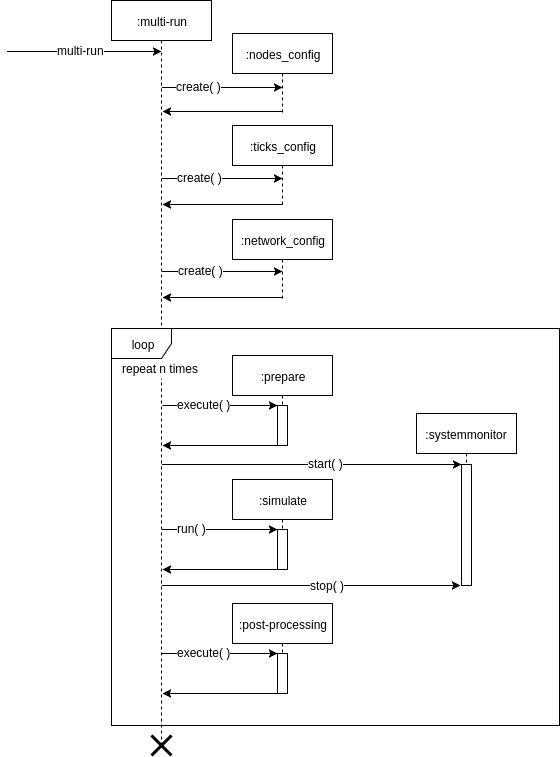
\includegraphics[width=8cm]{flow_chart_multi_run}
\centering
\caption{Sequence diagram of the \textit{multi-run} command}
\label{fig:flow_chart_multi_run}
\end{figure}

\subsection{\textit{multi-run} command} \label{chap:multi_run_command}

The \textit{multi-run} command accepts an input parameter denoting how often a run should be repeated ($repeat$).
The simulation framework then creates all configuration files using the passed input arguments and subsequently executes the simulation $repeat$ times using the same configuration files as depicted in figure \ref{fig:flow_chart_multi_run}.

\section{Long-term storage of simulation data}

During a simulation run, all nodes persist their data on the disk of the host machine.
Most of the persisted data by a node are the blocks created during the simulation scenario.
Since all nodes act independently, these blocks are furthermore replicated multiple times on the host.
Thus, the amount of simulation data can be very large occupying multiple gigabytes on the host disk.
To reduce the needed space for a long-term storage the replicated blocks can be deduplicated by using the file system \textit{ZFS}.
The usage of deduplication trades off with a slower performance when persisting or retrieving files from a \textit{ZFS} system.
Hence, a \textit{ZFS} file system may not be used during a simulation where a slow file system could impact the results of a simulation.

To use deduplication for the created blocks the method to store the blocks is crucial.
The nodes involved in the simulation persist their blocks in files with the name \textit{blk*.dat}, where the \textit{*} is an ongoing file number.
These \textit{blk-files} have a fixed size and whenever a file is full a new file is allocated starting initially with one single file.
During the simulation, the node persists the blocks according to their arrival order.
Hence, the arrangement of the blocks in the files can vary between the nodes, because the blocks can arrive with a different order at a node.
For example, when a fork happens, some nodes will persist block \textit{A} as next block, where other nodes will persist the competing block \textit{B} which results in different \textit{blk-files} between the nodes.
These differing \textit{blk-files} cannot be deduplicated by \textit{ZFS} even though they contain the same blocks of the simulation.
If \textit{ZFS} is configured to deduplicate newly stored files, it internally splits the files according to a pre-defined block size (to avoid confusion this block sizes will be called \textit{ZFS-block-size}) and checks if this block (\textit{ZFS-block}) is already stored by the file system.
In the case that the \textit{ZFS-block} is already stored, \textit{ZFS} stores for the inserted file a reference to this block.
In the other case where the ZFS-block is not known, \textit{ZFS} stores the new block and updates an internal table denoting the presence of this \textit{ZFS-block}.
Hence, to fully deduplicate all blocks available multiple times in the \textit{blk-files}, the blocks need to be aligned with a multiple of the \textit{ZFS-block-size}.

\begin{minipage}{\linewidth}
\begin{lstlisting}[caption=Aligning the block size in the Bitcoin reference implementation for \textit{ZFS}, label={lst:align_zfs}, basicstyle=\ttfamily, captionpos=b]
unsigned int nextPowerOfTwoExponent
	= ceil(log2(nBlockSize + 8));
unsigned int nextPowerOfTwo
	= nextPowerOfTwoExponent > 9?
		pow(2, nextPowerOfTwoExponent) : pow(2,9);
nBlockSize = nextPowerOfTwo - 8;
\end{lstlisting}
\end{minipage}

Listing \ref{lst:align_zfs} shows how this can be achieved in the Bitcoin reference implementation by setting the \textit{nBlockSize} in the file \textit{validation.cpp} to the next power of two.
The blocks persisted by nodes implementing the introduced patch are then occupying a power of two big space in the used \textit{blk-file}.
If now the \textit{ZFS} file system persists a \textit{blk-file} all blocks are aligned and can be deduplicated if they are already stored in the file system.
The added and subtracted eight bytes in line 2 and 6 are an implementation detail in the Bitcoin reference implementation.
